\begin{frame}{IoT}

\centering
\Large{IoT with python and Raspberry Pi}\\
\textbf{PyDelhi 2016}
	
\end{frame}

\begin{frame}{Instructor}
	\begin{figure}
		\centering
		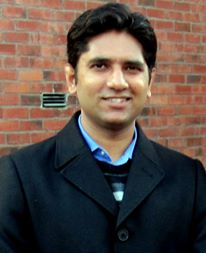
\includegraphics[width=4cm,height=4cm,keepaspectratio]{me}
	\end{figure}
	
	\centering
	\textcolor{blue}{Dr. Sandeep Nagar} \\
	M.Sc. Physics (MSU, Vadodara) \& PhD in Material Science \\ (Department of Material Science and Engineering, KTH, Sweden) \\
	contact e-mail: \textcolor{red}{sandeep.nagar@gmail.com}
\end{frame}

\begin{frame}{Why would I do IoT?}
	\begin{itemize}
		\item Its for everybody!
		\item Started just for fun
		\item Some serious experimentation
		\item Making scientific instruments
		\item Internet control gives multi-functionality to experiments
	\end{itemize}
\end{frame}

\begin{frame}{Outline of workshop}
	\begin{enumerate}
		\item Introduction to Raspberry Pi ($30$ Minutes)
		\begin{itemize}
			\item Various parts
			\item Installing OS
		\end{itemize}
		\item Accessing GPIO pins ($30$ minutes)
		\begin{itemize}
			\item Writing to GPIO pins
			\item Reading from GPIO pins
		\end{itemize}
		\item IoT with RPi ($30$ minutes)
		\begin{itemize}
			\item Running RPi headless 
			\item Adding sensors
			\item Interacting with data generated using IoT device
		\end{itemize}
	\end{enumerate}
\end{frame}

\begin{frame}{title}
	content...
\end{frame}